\documentclass[11pt]{article}
\usepackage[margin=0.72in,headheight=15pt]{geometry}
\usepackage{graphicx}
\usepackage{booktabs}
\usepackage{array}
\usepackage{tabularx}
\usepackage{longtable}
\usepackage{amsmath}
\usepackage{xcolor}
\usepackage{hyperref}
\usepackage{fancyhdr}
\usepackage{float}
\usepackage{caption}
\usepackage{enumitem}
\usepackage{microtype}

\definecolor{navy}{HTML}{17324D}
\definecolor{teal}{HTML}{168C91}
\definecolor{lightblue}{HTML}{EDF5FA}
\hypersetup{
  colorlinks=true,
  linkcolor=navy,
  urlcolor=teal,
  pdftitle={Phase 4: Bearing-Aided EKF Localization},
  pdfauthor={Shakib Al Sifat},
  pdfsubject={Advanced Robotics (SCE 672)}
}
\pagestyle{fancy}
\fancyhf{}
\lhead{Advanced Robotics | Phase 4}
\rhead{Bearing-Aided EKF Localization}
\cfoot{\thepage}
\setlength{\parskip}{5pt}
\setlength{\parindent}{0pt}
\captionsetup{font=small,labelfont=bf}
\graphicspath{{report_figures/}}

\begin{document}

% Cover page
\begin{titlepage}
\thispagestyle{empty}
\centering
\vspace*{\fill}
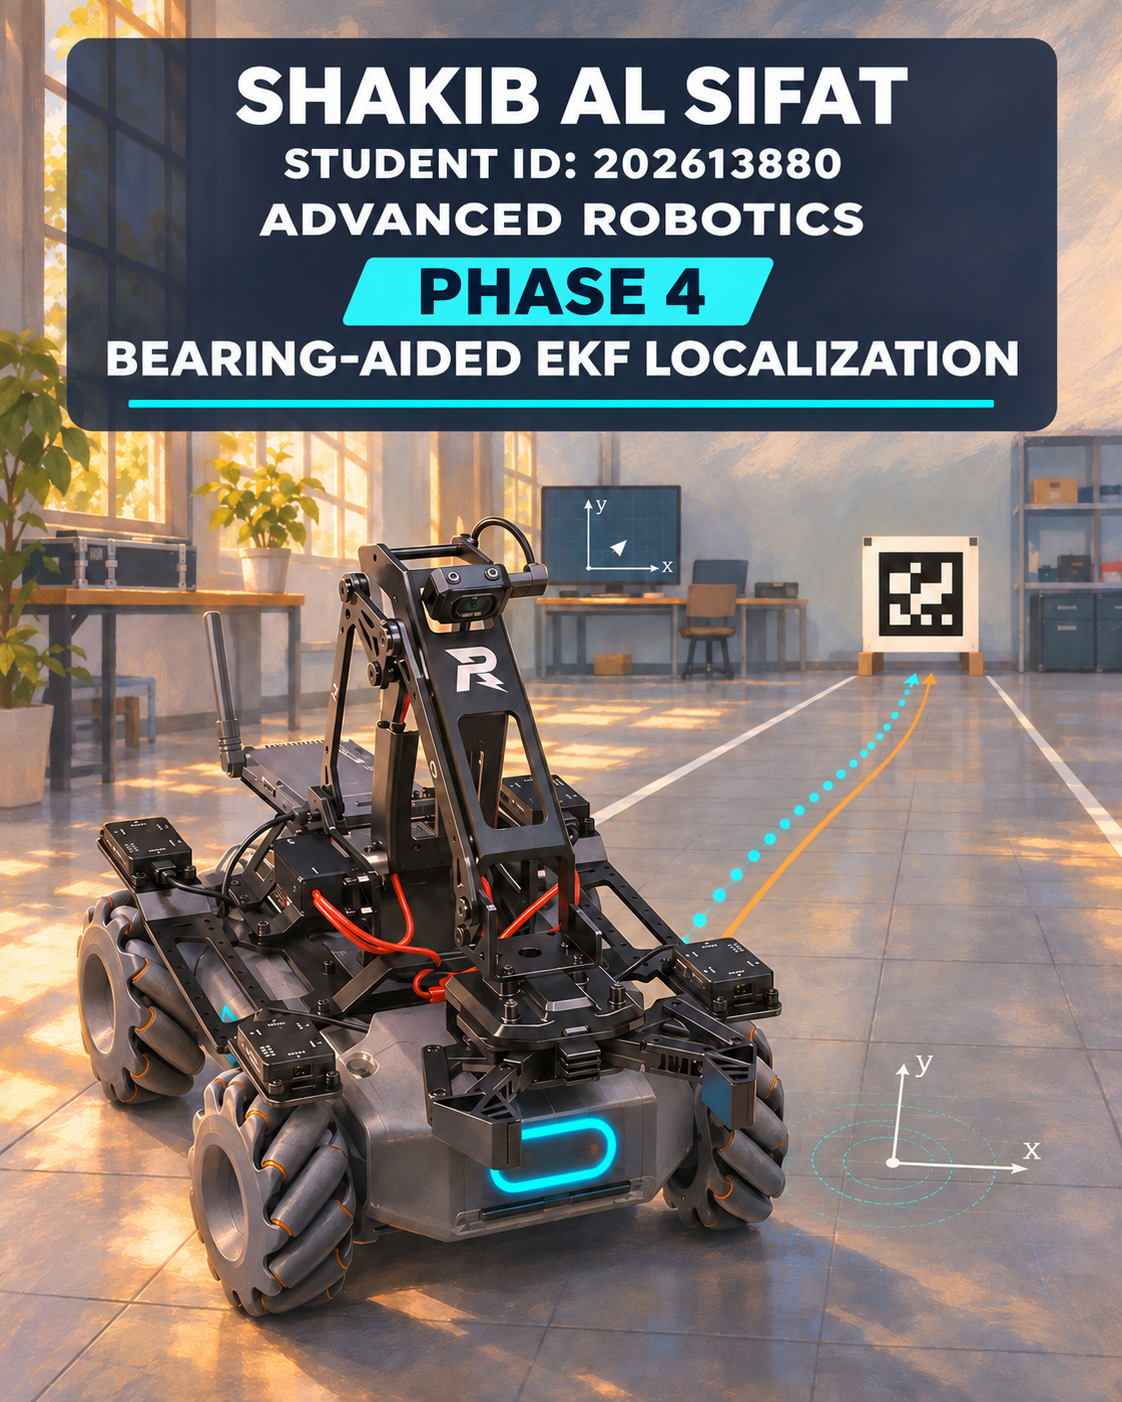
\includegraphics[width=0.82\textwidth,height=0.93\textheight,keepaspectratio]{../output/covers/cover_page.png}
\vspace*{\fill}
\end{titlepage}

\begin{center}
{\LARGE\bfseries\color{navy} Phase 4: Bearing-Aided EKF Localization}\\[4pt]
{\large Advanced Robotics (SCE 672)}\\[8pt]
{\large Shakib Al Sifat \quad | \quad Student ID: 202613880}\\
King Fahd University of Petroleum and Minerals\\
November 2026
\end{center}

\section*{Executive Summary}
In this project, I evaluated whether camera-based bearing measurements to a fixed AprilTag could improve the RoboMaster EP Core's straight-line position estimate when combined with chassis odometry in an Extended Kalman Filter (EKF). I ran eight fixed-start trials and compared the final odometry and EKF positions with my tape-measured chassis-center endpoints. The mean Euclidean endpoint error was 3.30 cm for odometry and 6.00 cm for the EKF. With the current setup and provisional noise values, the bearing updates did not improve endpoint accuracy and introduced a consistent leftward bias in the EKF estimates.

\textbf{Submission links:} \href{https://github.com/ssifat109/robomaster-odometry-phase3/tree/main/phase4}{Phase 4 project files on GitHub} \quad | \quad \href{https://youtube.com/shorts/OIwx5EAHnV4}{All-trials side-by-side video on YouTube}.

\section{Objective and Experimental Setup}
I used the camera bearing to a stationary landmark as a measurement that could correct position and heading estimates propagated from the robot's odometry. I drove the robot forward along a straight floor path while keeping the AprilTag to the left of the path.

I marked the origin at the chassis center and used +x for forward travel, +y for left, and an initial heading of zero along the path. I placed the tag approximately 1.20 m ahead and 0.40 m left of the robot camera. The camera was approximately 0.03 m ahead of the chassis-center origin, so I used a tag-center coordinate of (1.17 m, 0.40 m) in the chassis floor frame. I used a 142 mm black-square AprilTag 36h11, ID 3, and kept the camera/gimbal fixed.

\begin{table}[H]
\centering
\caption{Experimental settings used in the analyzed runs.}
\begin{tabularx}{\linewidth}{>{\bfseries}p{0.27\linewidth} X}
\toprule
Item & Setting \\
\midrule
Robot and connection & RoboMaster EP Core; DJI SDK, AP connection \\
Motion command & Straight forward; 0.10 m/s commanded speed for 13.5 s \\
Nominal travel & Approximately 1.35 m; actual travel varied between runs \\
Coordinate frame & Origin at initial chassis center; +x forward; +y left \\
Landmark & AprilTag 36h11, ID 3; 0.142 m measured black-square edge \\
Tag center in configuration & (1.17 m, 0.40 m) \\
Camera configuration & x offset -0.03 m; yaw correction 0.0271 rad \\
Ground truth & Independent tape measurement of the final chassis-center position \\
\bottomrule
\end{tabularx}
\end{table}

Before I ran the trials, I checked the camera while the robot was stationary. The detector found ID 3 in 357 of 357 frames. Its mean bearing was 17.27 degrees, compared with the configured geometry prediction of 16.88 degrees. I treated the small frame-to-frame variation as repeatability only, not as an independent absolute calibration.

\begin{figure}[H]
\centering
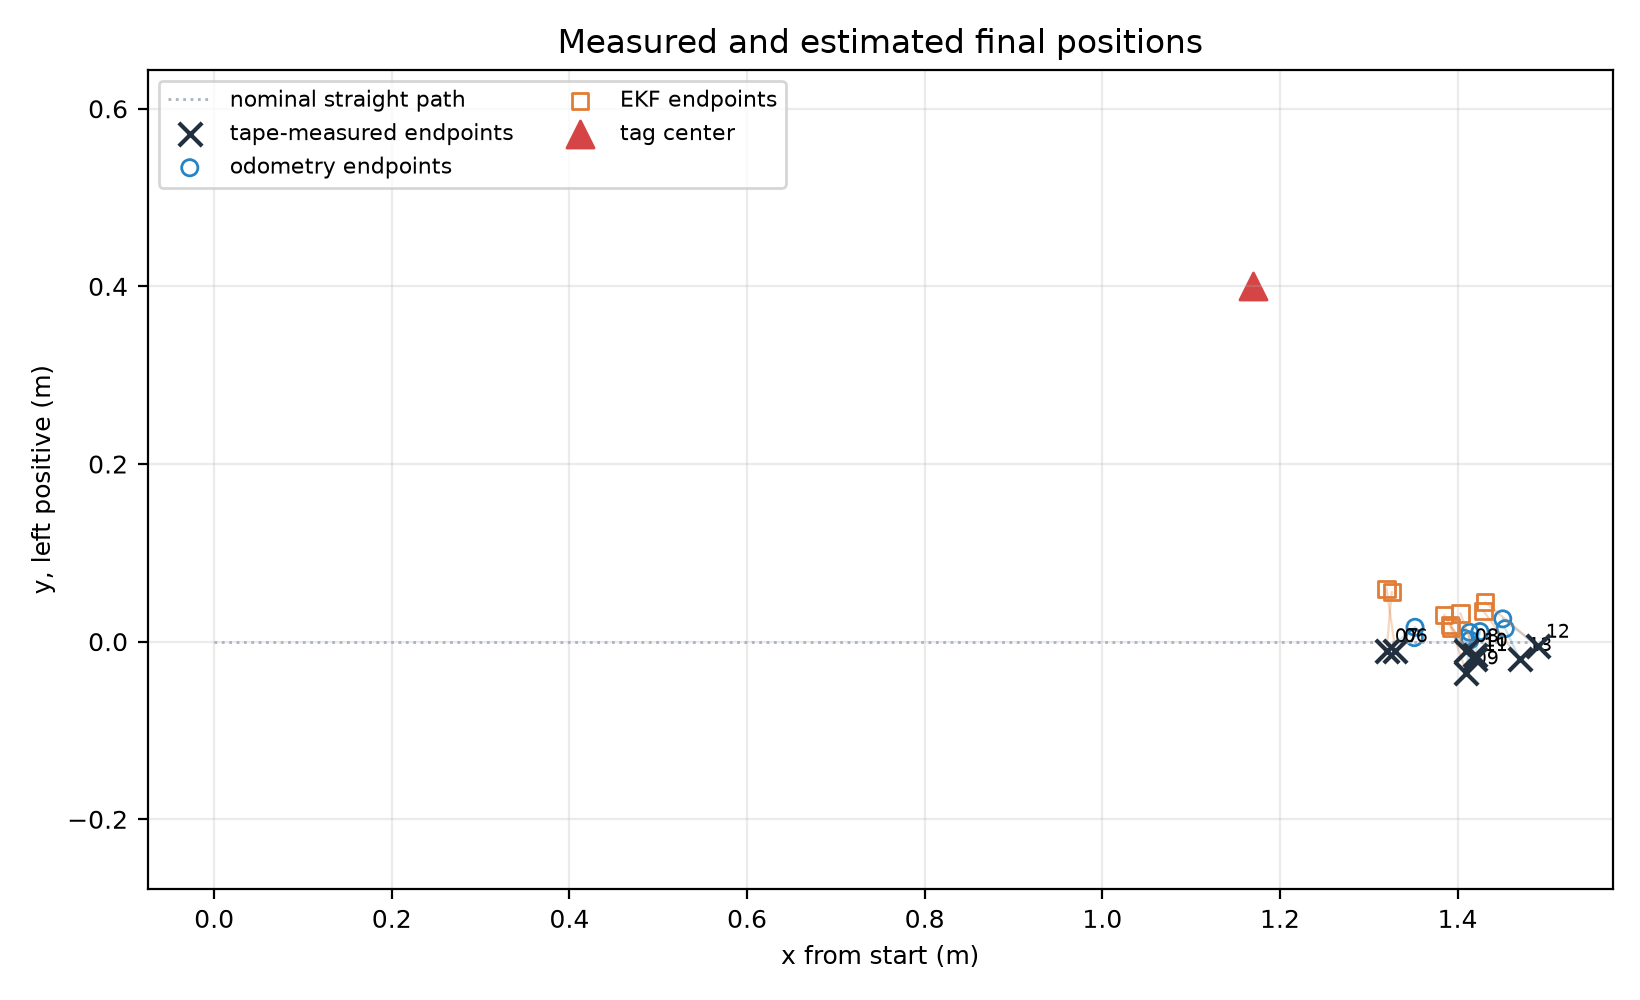
\includegraphics[width=0.88\linewidth]{endpoints.png}
\caption{Tape-measured endpoints compared with the odometry and EKF estimates. The triangle marks the tag center.}
\end{figure}

\section{Localization Method}
I represented the robot pose as $\mathbf{x}=[x,y,\theta]^T$. At each odometry step, I rotated the body-frame forward and lateral increments into the experiment frame:
\begin{align}
x_{k+1} &= x_k + \cos\theta_k\,\Delta x_b - \sin\theta_k\,\Delta y_b,\\
y_{k+1} &= y_k + \sin\theta_k\,\Delta x_b + \cos\theta_k\,\Delta y_b,\\
\theta_{k+1} &= \operatorname{wrap}(\theta_k+\Delta\theta).
\end{align}
For the bearing update, I used the camera observation of the fixed tag. In simplified form, the predicted bearing is
\begin{equation}
h(\mathbf{x})=\operatorname{atan2}(y_t-y,\,x_t-x)-\theta-\psi_c,
\end{equation}
where $(x_t,y_t)$ is the tag center and $\psi_c$ is the configured camera yaw correction. I also included the configured camera translation in the bearing geometry.

I propagated covariance with $P^- = FPF^T+Q$. For each bearing observation, I formed the innovation covariance $S=HP^-H^T+R$ and Kalman gain $K=P^-H^TS^{-1}$. I used the Joseph covariance update, $P=(I-KH)P^-(I-KH)^T+KRK^T$, and wrapped angular differences to $[-\pi,\pi)$. For the odometry-only comparison, I propagated the initial position with odometry and did not apply bearing updates.

\section{Noise Assumptions}
I used the values in Table~\ref{tab:noise} as provisional starting assumptions. I did not estimate them from dedicated repeated-motion and independent bearing-calibration datasets, so I do not interpret them as measured sensor specifications.

\begin{table}[H]
\centering
\caption{Configured process and bearing noise.}
\label{tab:noise}
\begin{tabularx}{\linewidth}{p{0.31\linewidth}p{0.22\linewidth}p{0.18\linewidth}>{\raggedright\arraybackslash}X}
\toprule
Term & Standard deviation & Variance & Basis \\
\midrule
Forward odometry increment & 7 mm/sample & $4.9\times10^{-5}$ m$^2$ & Provisional setting \\
Lateral odometry increment & 7 mm/sample & $4.9\times10^{-5}$ m$^2$ & Provisional setting \\
Heading increment & 0.5 degrees/sample & $7.62\times10^{-5}$ rad$^2$ & Provisional setting \\
Camera bearing & 3 degrees & $2.74\times10^{-3}$ rad$^2$ & Conservative provisional setting \\
\bottomrule
\end{tabularx}
\end{table}

I calculated the reported one-sigma position values as the square roots of the final covariance diagonal entries. They describe uncertainty under my configured model. Since the residuals show a directional bias, I do not treat these values as capturing every source of observed error.

\section{Results}
I analyzed trials 06 through 13. Table~\ref{tab:trials} lists each measured endpoint, each estimated endpoint, the Euclidean errors, and the final EKF standard deviations. Positions and errors are in metres; $y$ is positive to the left.

\begin{table}[H]
\centering
\caption{Per-trial final positions and errors (metres).}
\label{tab:trials}
\scriptsize
\resizebox{\linewidth}{!}{%
\begin{tabular}{c r r r r r r r r r r}
\toprule
Trial & Actual x & Actual y & Odom x & Odom y & EKF x & EKF y & Odom err. & EKF err. & $\sigma_x$ & $\sigma_y$ \\
\midrule
06 & 1.330 & -0.010 & 1.351 & 0.005 & 1.320 & 0.060 & 0.026 & 0.070 & 0.076 & 0.071 \\
07 & 1.320 & -0.010 & 1.352 & 0.016 & 1.326 & 0.056 & 0.041 & 0.066 & 0.076 & 0.071 \\
08 & 1.410 & -0.010 & 1.407 & 0.004 & 1.385 & 0.030 & 0.014 & 0.047 & 0.080 & 0.077 \\
09 & 1.410 & -0.035 & 1.414 & 0.010 & 1.393 & 0.016 & 0.046 & 0.054 & 0.081 & 0.078 \\
10 & 1.420 & -0.015 & 1.425 & 0.011 & 1.403 & 0.032 & 0.027 & 0.050 & 0.081 & 0.078 \\
11 & 1.420 & -0.020 & 1.414 & 0.002 & 1.391 & 0.019 & 0.023 & 0.048 & 0.080 & 0.077 \\
12 & 1.490 & -0.005 & 1.451 & 0.026 & 1.431 & 0.044 & 0.050 & 0.077 & 0.081 & 0.079 \\
13 & 1.470 & -0.020 & 1.454 & 0.015 & 1.429 & 0.034 & 0.038 & 0.068 & 0.080 & 0.079 \\
\bottomrule
\end{tabular}}
\end{table}

\begin{table}[H]
\centering
\caption{Aggregate comparison across the eight analyzed trials.}
\begin{tabular}{lrr}
\toprule
Measure & Odometry & EKF \\
\midrule
Mean absolute x error & 1.58 cm & 2.54 cm \\
Mean absolute y error & 2.67 cm & 5.19 cm \\
Mean signed x residual & -0.02 cm & -2.40 cm \\
Mean signed y residual & 2.67 cm & 5.19 cm \\
Mean Euclidean error & 3.30 cm & 6.00 cm \\
Euclidean RMSE & 3.50 cm & 6.09 cm \\
Mean final $\sigma_x$ / $\sigma_y$ & -- & 7.94 / 7.62 cm \\
Coordinate residuals within $1\sigma$ & -- & x: 8/8; y: 8/8 \\
\bottomrule
\end{tabular}
\end{table}

\begin{figure}[H]
\centering
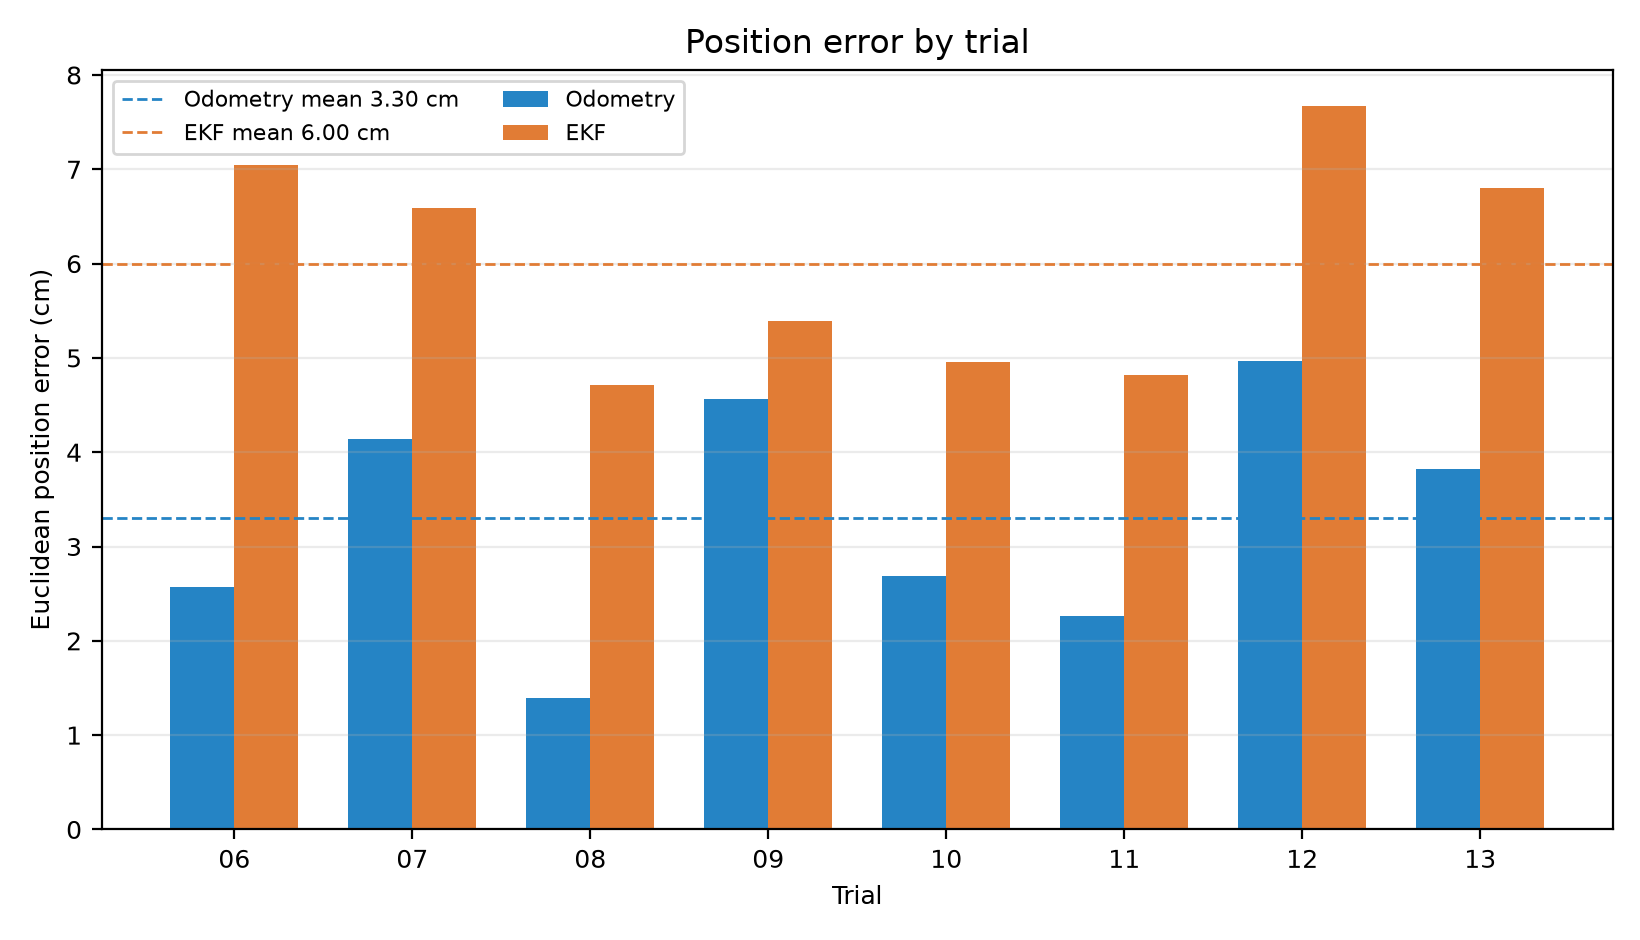
\includegraphics[width=0.84\linewidth]{position_errors.png}
\caption{Euclidean endpoint error by trial. Dashed lines show the method means.}
\end{figure}

\begin{figure}[H]
\centering
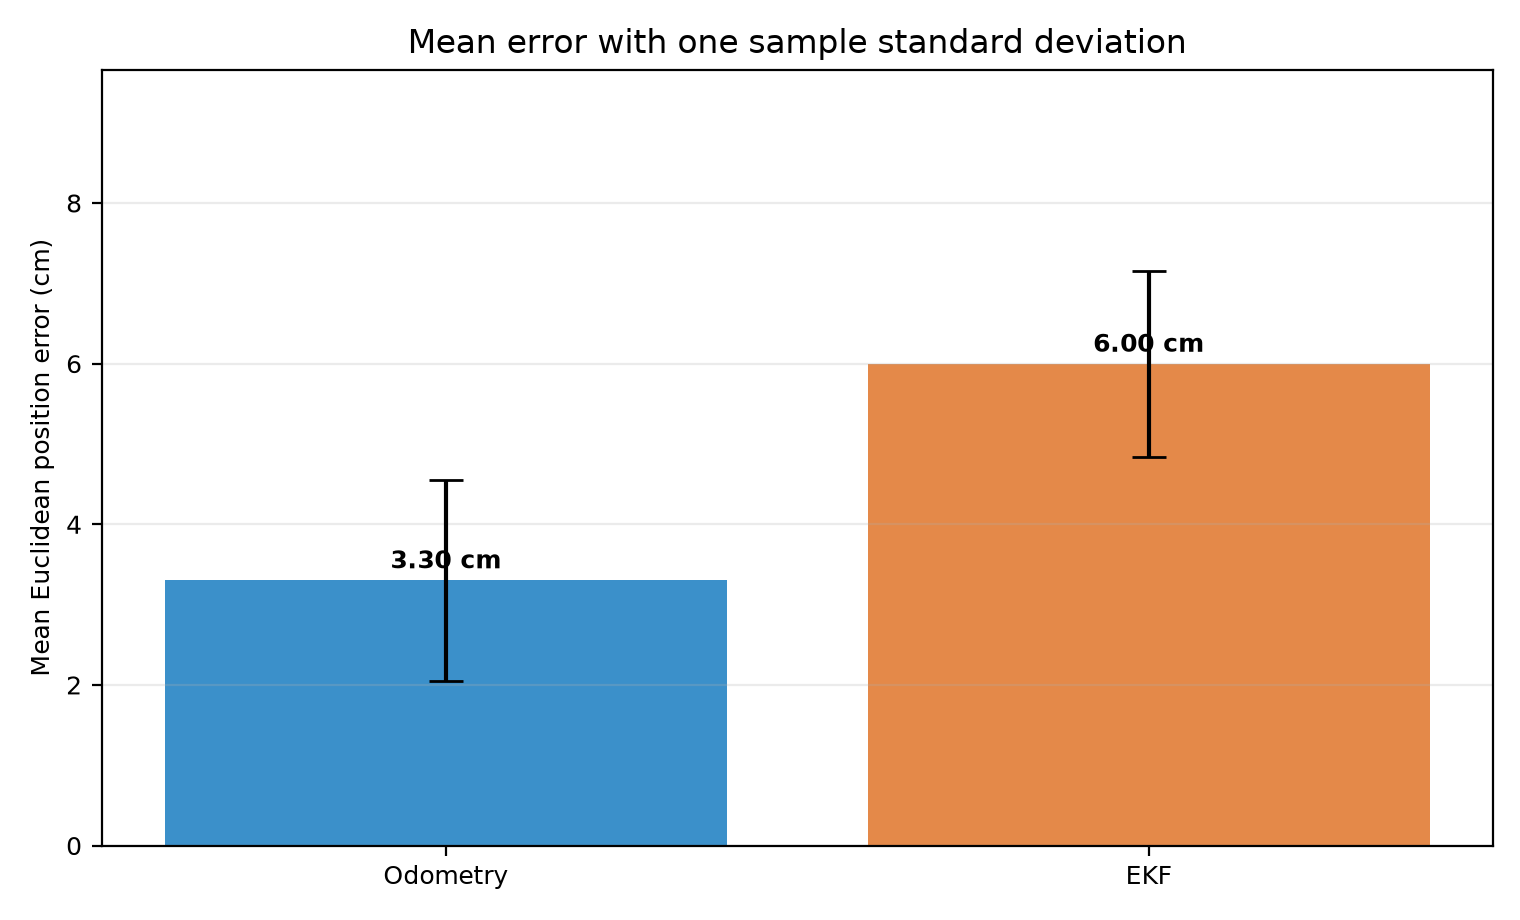
\includegraphics[width=0.78\linewidth]{mean_error.png}
\caption{Mean Euclidean error with one sample standard deviation across trials.}
\end{figure}

\begin{figure}[H]
\centering
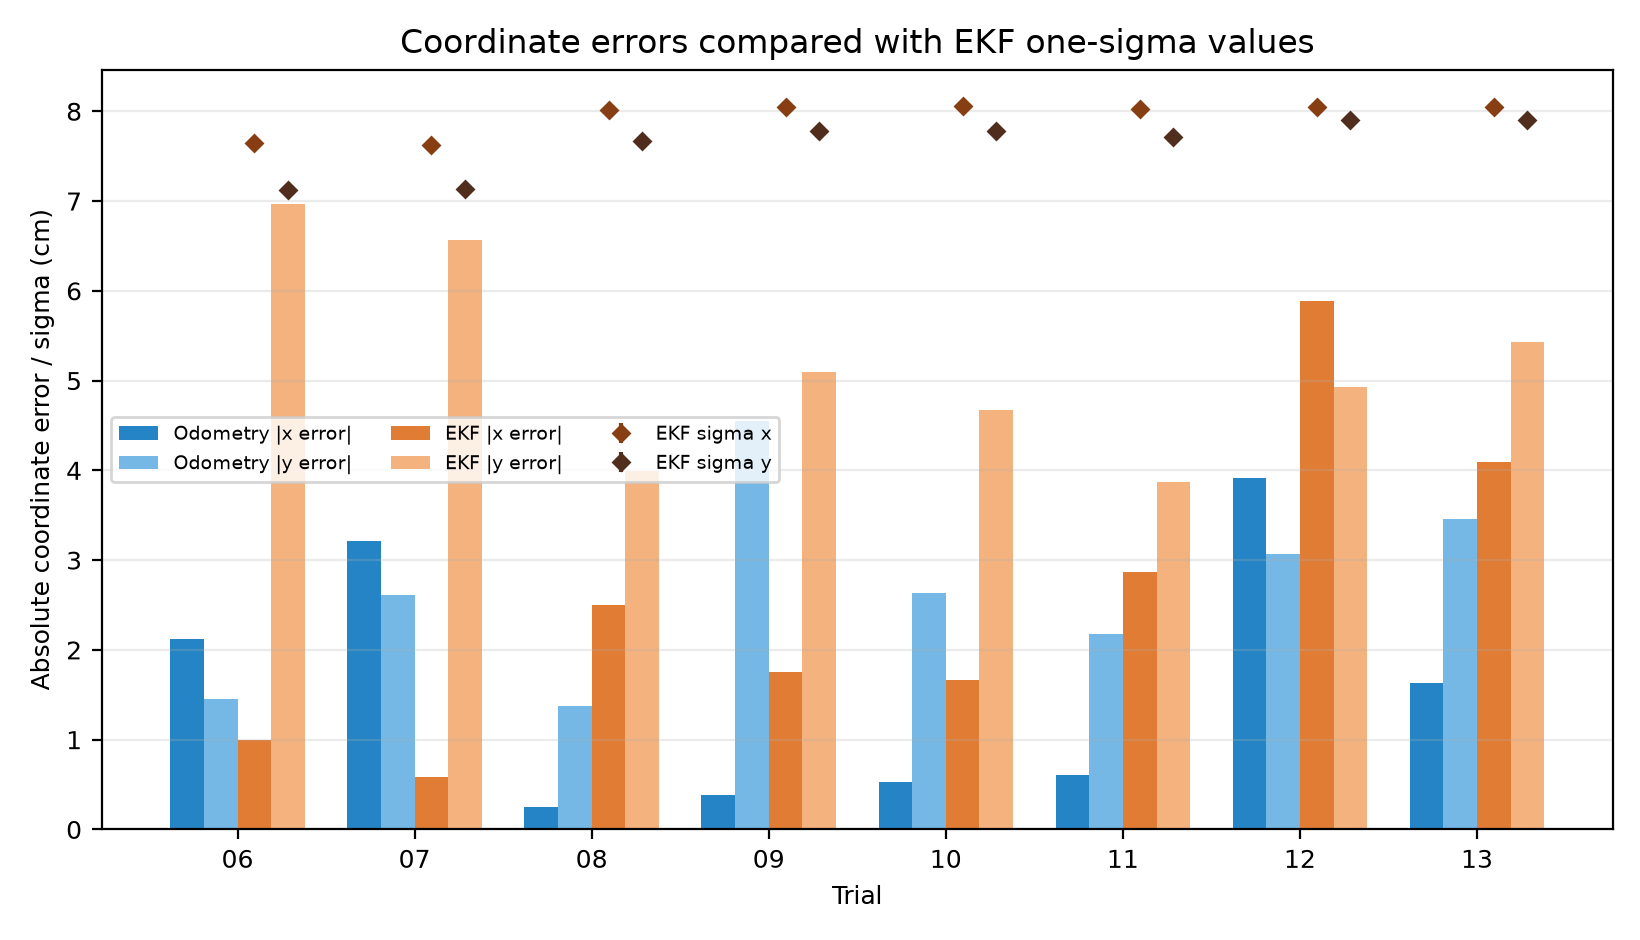
\includegraphics[width=0.88\linewidth]{coordinate_sigma.png}
\caption{Absolute coordinate residuals and final EKF one-sigma values.}
\end{figure}

\begin{figure}[H]
\centering
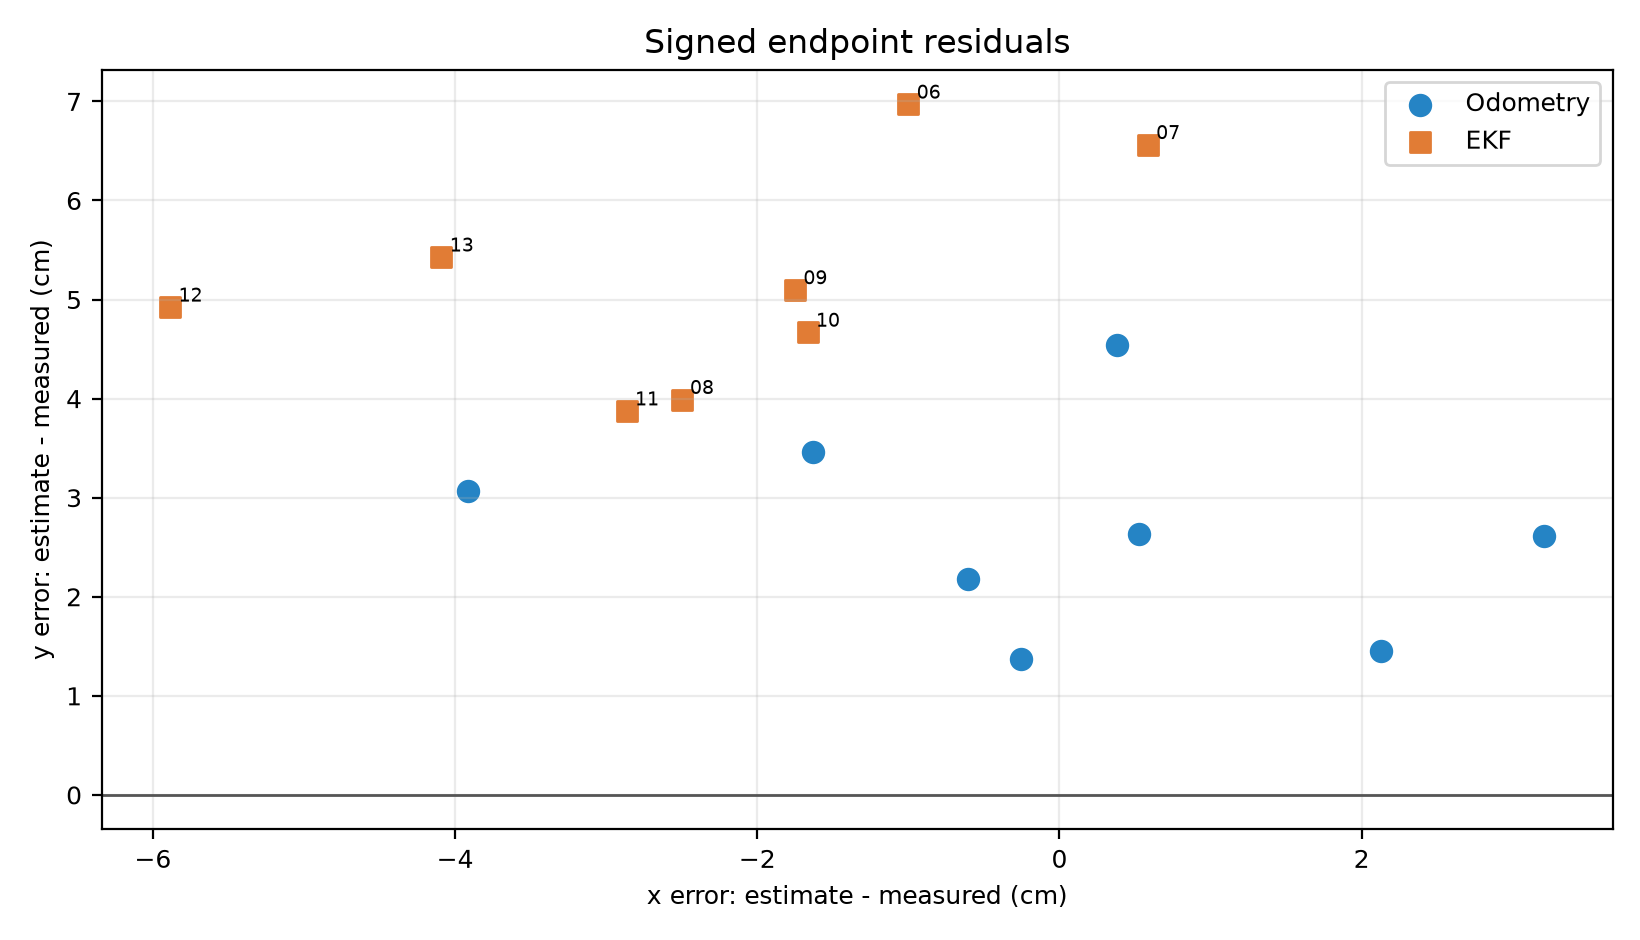
\includegraphics[width=0.82\linewidth]{residuals.png}
\caption{Signed endpoint residuals, computed as estimate minus tape measurement.}
\end{figure}

\begin{figure}[H]
\centering
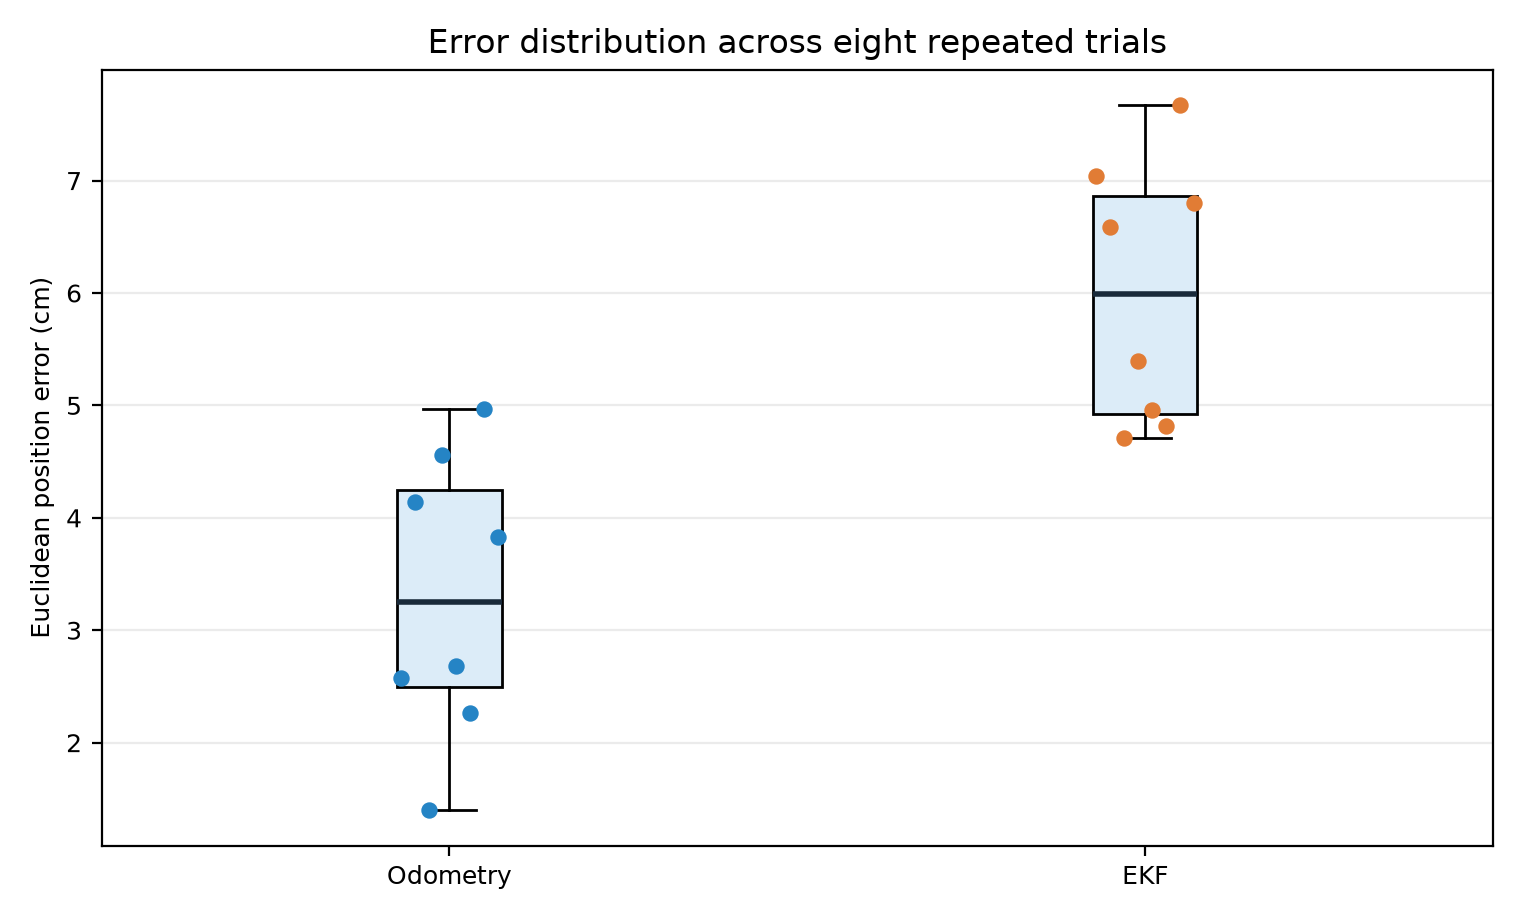
\includegraphics[width=0.74\linewidth]{error_distribution.png}
\caption{Distribution of Euclidean errors. With eight trials, I treat these summaries descriptively.}
\end{figure}

\begin{figure}[H]
\centering
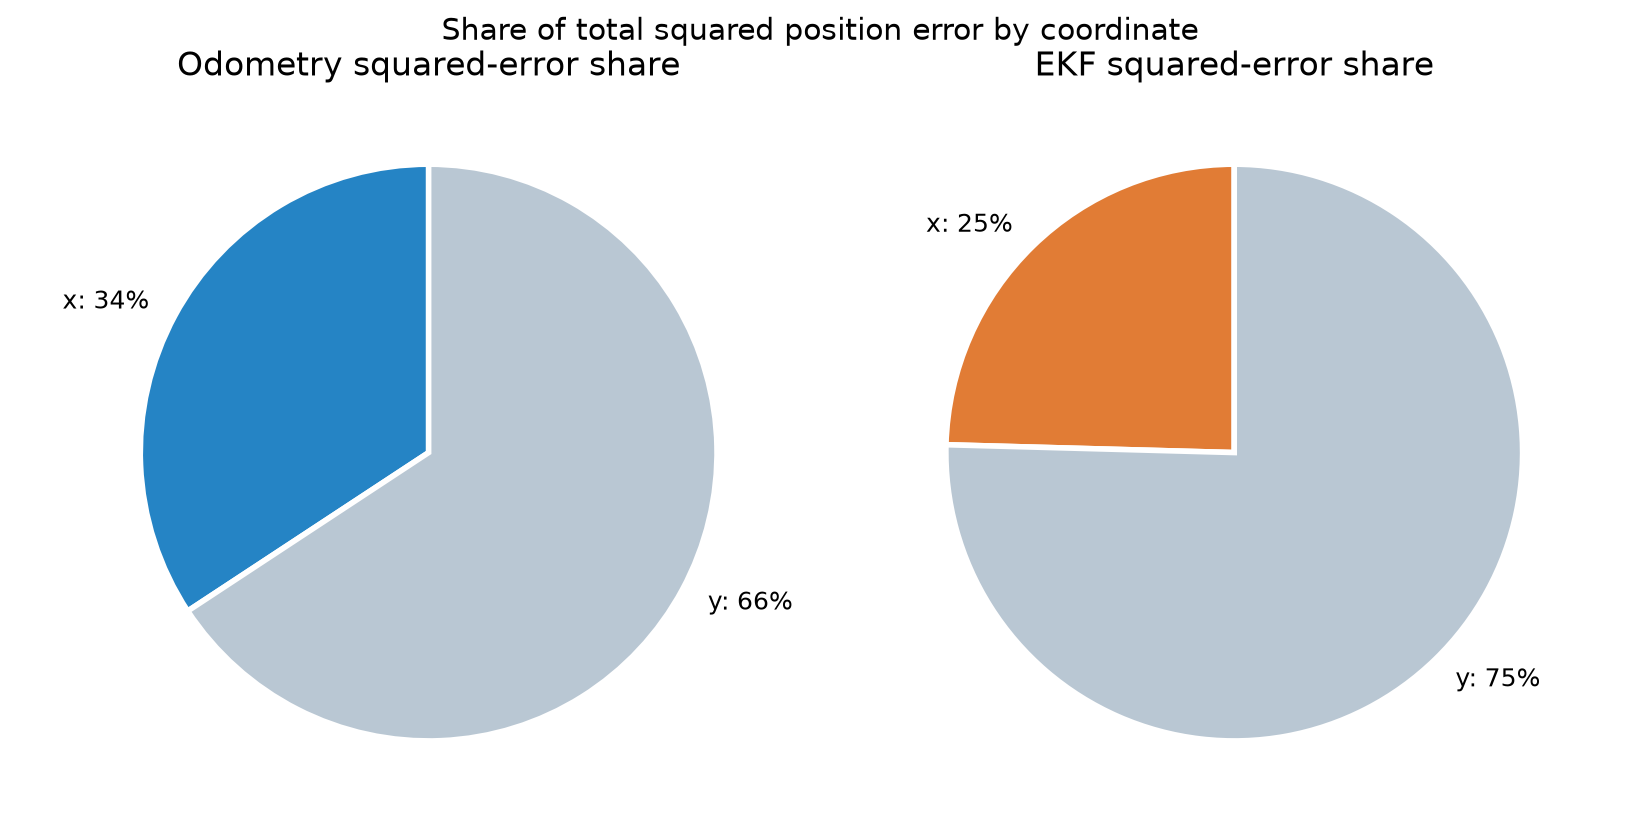
\includegraphics[width=0.82\linewidth]{error_share.png}
\caption{Share of summed squared endpoint residual attributable to x and y for each method.}
\end{figure}

\section{Discussion and Limitations}
Across these runs, I found that the bearing update did not improve the endpoint estimate: mean error increased from 3.30 cm for odometry to 6.00 cm for the EKF. The EKF's mean signed y residual was +5.19 cm, meaning that its estimates were too far left on average in my coordinate frame. The same sign of lateral bias appeared in all eight final EKF estimates.

All eight x and y residual magnitudes were within the final one-sigma values reported by the EKF. I do not treat this as evidence that the uncertainty is calibrated. I used provisional $Q$ and $R$ values, the sample contains only eight trials, and the EKF residuals have a clear directional bias.

I see several possible sources of error: camera intrinsic and yaw calibration, the tag and camera offsets, conversion from image position to bearing, camera/odometry timestamp alignment, yaw reference drift, wheel slip, start alignment, and tape-measure precision. The final forward distance also varied between runs, so the trials represent a repeated setup and command rather than identical realized travel. I would next survey the camera and tag geometry, estimate bearing noise from independent poses, and estimate odometry noise from repeated controlled motion before retuning $Q$ and $R$.

\section{Trial Selection and Submitted Video}
I used trials 06--13 for the quantitative comparison because they share the fixed-start setup and have independent endpoint measurements. I excluded trials 01, 03, and 04 because they were earlier setup attempts and did not provide comparable ground truth for this series. Trial 02 failed during startup before it produced a valid run. I excluded trial 05 because I could not confirm its endpoint and starting setup were comparable with the fixed-start trials. I left those attempts out of the statistics, but they are included in my combined video.

I combined the phone footage and the RoboMaster camera footage side by side into one video containing all trial attempts. I posted the combined video at \href{https://youtube.com/shorts/OIwx5EAHnV4}{YouTube - all trial runs}.

\section{Reproducibility and Project Files}
I included the analysis source, filter configuration, trial logs for runs 06--13, result tables, figures, cover image, and report source in the Phase 4 GitHub folder. I uploaded the full project to \href{https://github.com/ssifat109/robomaster-odometry-phase3/tree/main/phase4}{the Phase 4 GitHub folder}. The LaTeX source for this report is included alongside the report outputs.

\end{document}







